\chapter{Vývoj zařízení - Komponenty}
\label{4-vyvoj-zarizeni-komponenty}
\section{Vývojová deska}
Vývojová deska je elektronické zařízení skládající se z~desky plošných spojů, mikro\-kontroléru a k~němu připojených dalších periférií. Mikrokontrolér je malý \text{počítač} na jednom integrovaném obvodu, který může obsahovat jedno nebo více jader \text{procesoru}, paměť pro uložení programu, operační paměť a programovatelné \text{vstupy/výstupy}. Mikrokontrolér neobsahuje operační systém a řídící program na něj bývá nahraný \text{pomocí} integrovaného vývojového prostředí (\zk{IDE}, z~anglického Integrated Develop\-ment Environment). Mikrokontrolér ovládá k~němu připojené periférie a další součástky připojnené k~vývojové desce. Připojením součástek k~vývojové desce lze vytvořit nové elektronické zařízení \cite{dps_vyvojove_desky}.

\subsection{Arduino Uno}
Jako vývojová deska bylo zvoleno Arduino UNO, a to z~důvodu jeho poměrně nízké ceny, velkého množství dostupné dokumentace a kompatibilních součástek. Tato vývojová deska, na které je nahraný řídící program, ovládá všechny ostatní použité komponenty. Nejběžněji se lze setkat s~Arduinem UNO R3, které je \text{založené} na mikrokontroléru ATmega328P od firmy Atmel. Z~důvodu malé kapacity paměti \text{Arduina} UNO R3 bylo využito novější Arduino UNO R4. To je založeno na mikrokontroléru Renesas RA4M1, jenž obsahuje procesor ARM Cortex-M4F. Arduino UNO R4 se vyrábí ve verzích Minima a WiFi. Verze WiFi je zaměřena na IoT aplikace a obsahuje navíc mikrokontrolér ESP32-S3 od firmy Espressif s~integrovaným WiFi a bluetooth low energy (BLE) modulem. Toho lze využít pro připojení k~NTP serveru, nebo odesílání dat \cite{arduino}. Arduino UNO lze pořídit i v~podobě „klonu“, který vyrábí neoficiální výrobce. Tyto „kolny“ bývají obvykle cenově dostupnější než \text{originální desky}.

% https://www.robotikabrno.cz/docs/arduino/Pr%C5%AFvodce-sv%C4%9Btem-Arduina-CZ.pdf

\begin{table}[H]
    \centering
    \caption{Porovnání kapacity paměti Arduina UNO R3 a R4 \cite{arduino}}
    \begin{tabular}{|c|c|c|}
    \hline
    \textbf{Typ paměti} & \textbf{R3} & \textbf{R4}\\
    \hline\hline
    flash  & 32 KB & 256 kB \\ \hline
    SRAM   & 2  KB &  32 kB \\ \hline
    EEPROM & 1  KB &   8 kB \\ \hline
    \end{tabular}\\
\end{table}

\begin{figure}[H]
	\centering
	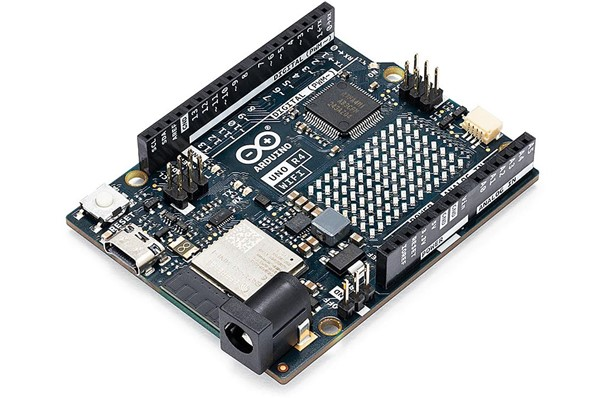
\includegraphics[width=6.5cm]{images/komponenty/UNO_R4.jpg}
	\caption{Arduino UNO R4 ve verzi WiFi \cite{laskakit_web}}
\end{figure}


\subsection{Arduino Mega}
Vzhledem k~nedostatečné kapacitě paměti Arduina UNO R3 se rovněž nabízí možnost využití Arduina Mega. To je založené na mikrokontroléru ATmega2560. Oproti \text{Arduinu} UNO R3 disponuje větší kapacitou paměti, a oproti oběma verzím Arduina UNO i větším množstvím pinů. Nevýhodou Arduina Mega je větší fyzická velikost a bylo tedy využito jen pro testování během vývoje zařízení \cite{arduino}.


\begin{figure}[H]
	\centering
	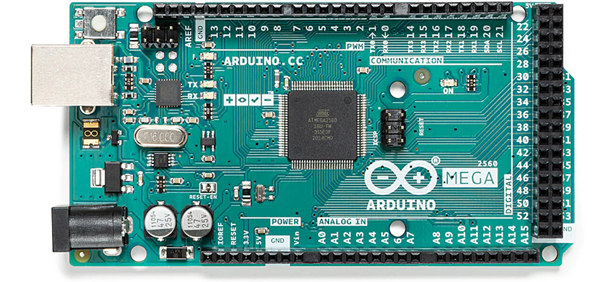
\includegraphics[width=6.5cm]{images/komponenty/mega.png}
	\caption{Arduino Mega \cite{arduino}}
\end{figure}

\section{Přijímač časového signálu}
Existuje několik způsobů, jak synchronizovat čas Arduina s~koordinovaným časem. Jedním z~nich je synchronizace času při nahrávání programu do Arduina. Tato metoda však vyžaduje opakované nahrání programu před každým měřením, aby se interní čas aktualizoval. Tato metoda neumožňuje průběžnou synchronizaci a její přesnost je závislá na přesnosti vnitřního času zařízení z~nějž je program nahráván. Vhodnějšími metodami jsou synchronizace přes internet, využití přijímače DCF77, který přijímá koordinovaný čas pomocí rádiového signálu, nebo využití času z~NMEA zprávy z~GNSS přijímače. Tyto metody poskytují přesnější a průběžnou synchronizaci času bez nutnosti opakovaného nahrávání programu.

\subsection{Přijímač DCF77}
Pro příjem signálu DCF77 je vhodné zvolit anténu, která přijímá především magnetickou složku elektromagnetické vlny, protože elektrická složka vlny je citlivá na výšku antény nad povrchem a bývá výrazně více rušena okolním signálem z~jiných \text{elektronických} zařízení než magnetická složka. Pro příjem magnetické složky signálu lze využít rámovou anténu, která ale mívá poměrně velké rozměry. Obvykle se používá anténa o~průměru 0,5m. Z~důvodu kompaktnosti celého zařízení byla \text{zvolena} feritová anténa. Pokud by signál z~feritové antény nebyl dostatečně silný, je možné pro jeho zesílení přímo na feritovou anténu připojit rámovou anténu s~větším průměrem.

Využitý přijímač se skládá z~feritového jádra, kolem kterého je vinuta cívka a demodulátoru, který slouží k~oddělení modulačního signálu od nosného signálu. Anténa má dvě maxima a dvě minima. Pro příjem maximální intenzity signálu, je vhodné ji umístit kolmo na směr k~vysílači. Pokud by docházelo k~rušení signálu z~jednoho směru, lze to vyřešit tím, že bude anténa natočena minimem ke zdroji rušení \cite{fel_dcf77} \cite{vyvoj_hw_andel}.

\begin{figure}[H]
	\centering
	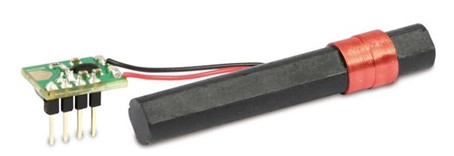
\includegraphics[width=6.1cm]{images/komponenty/DCF77_reciever.jpg}
	\caption{Přijímač radiového signálu DCF77 \cite{dratek_web}}
\end{figure}


\subsection{Přijímač GNSS}
Pro příjem informací o~aktuálním čase lze využít i GNSS přijímač. \text{Astrochrograf} je navržený tak, že má vyvedený pin D0 Arduina, aby k~němu mohl být \text{připojen} \text{libovolný} GNSS přijímač. Pin D0 na Arduinu Uno funguje jako RX pin pro \text{sériovou} komunikaci pomocí UART. GNSS přijímač musí být k~RX pinu Arduina \text{připojen} pomocí svého TX pinu. Přijímač musí poskytovat NMEA zprávu \$GNZDA, která obsahuje informace o~aktuálním čase a zprávu \$GNGGA, která poskytuje informaci o~poloze přijímače. Pro vývoj zařízení byl použit aktuálně dostupný GNSS \text{přijímač} Ublox NEO-M8T, který je schopen přijímat data ze satelitů GPS, GLONASS, Galileo, BeiDou, QZSS a SBAS. Tento přijímač umožňuje i RTK měření. Nevýhodou přijímače je poměrně vysoká cena. Pro určování času lze využít i přijímače s~omeze\-nější funkcionalitou než Ublox NEO-M8T. Například levnější přijímač Ublox NEO-M7M, který přijímá data ze satelitů GPS, GLONASS, Galileo a QZSS. Tento přijímač neumožňuje měření RTK, což není pro určování času potřeba.
\begin{figure}[H]
\centering
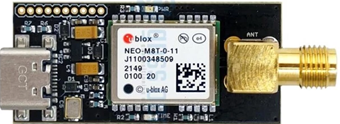
\includegraphics[width=6.1cm]{images/komponenty/GNSS_UBLOX.png}
\caption{GNSS přijímač Ublox NEO-M8T \cite{gnss_store}}
\end{figure}

\begin{figure}[H]
	\centering
	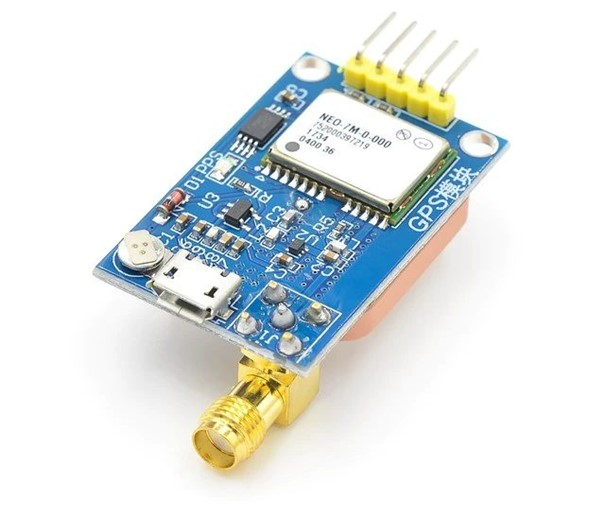
\includegraphics[width=6cm]{images/komponenty/UBLOX_NEO_7M.jpg}
	\caption{GNSS přijímač Ublox NEO 7M \cite{dratek_web}}
\end{figure}

\section{Čtečka Micro SD karet}
Protože Arduino samo o sobě nemá paměť pro ukládání dat, tak byla pro ukládání měřených dat využita Micro SD karta. Čtečka Micro SD karet umožňuje zapisovat měřená data na Micro SD kartu a popřípadě je z~ní i číst. Pro komunikaci s~čtečkou Micro SD karet je využíváno standardní SPI rozhraní \cite{arduino_navody}.

\begin{figure}[H]
	\centering
	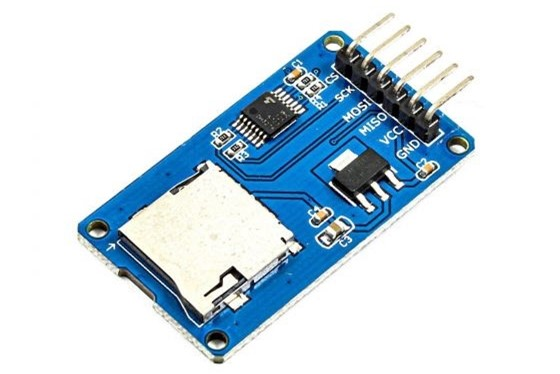
\includegraphics[width=6cm]{images/komponenty/ctecka_micro_sd.jpg}
	\caption{Čtečka Micro SD karet \cite{dratek_web}}
\end{figure}

\section{Tlačítko}
Tlačítko je jednoduchý komponent, sloužící pro detekci svého stisknutí. Stisknutí tlačítka slouží k~provedení záznamu času na Micro SD kartu. Místo samostatného tlačítka byl využit modul rotačního enkodéru, který umí detekovat své stisknutí a při pootočení osou poskytuje informaci o~směru rotace. Výhodou rotačního enkodéru oproti tlačítku je, že poskytuje další informace, které lze využít k~ovládání zařízení. Výhodou tohoto konkrétního modulu je to, že jej lze snadno upevnit ke krabičce s~výsledným zařízením.
\begin{figure}[H]
	\centering
	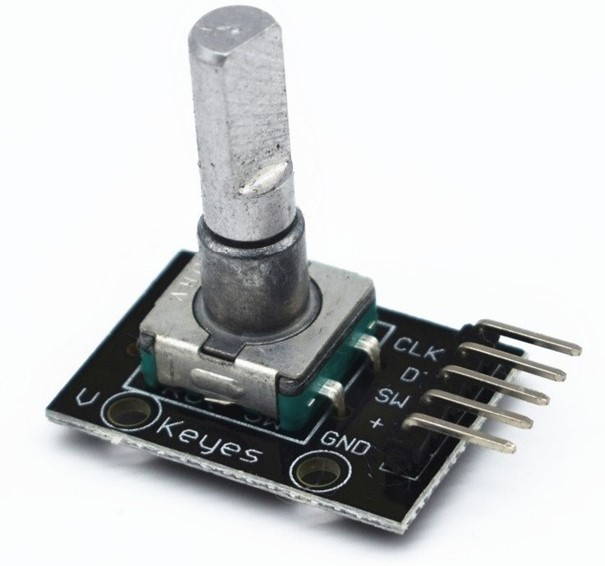
\includegraphics[width=4cm]{images/komponenty/rotacni_enkoder.jpg}
	\caption{Rotační enkodér \cite{dratek_web}}
\end{figure}

\section{OLED displej}
K~informování měřiče o~průběhu měření slouží mimo jiné displej. Na něj se zobrazuje informace o~stavu vložení Micro SD karty, o~stavu synchronizace času, aktuální čas a poslední uložený čas. Jako displej byl zvolen OLED displej především kvůli nízké ceně, dobré čitelnosti, nízké spotřebě energie a absenci potřeby dodatečného podsvícení, jelikož světélkují samotné pixely. Displej je monochromatický a jeho rozlišení je 128×64 bodů. K~řízení displeje je využívána komunikace pomocí I\(^2\)C sběrnice \cite{arduino_navody}.

\begin{figure}[H]
	\centering
	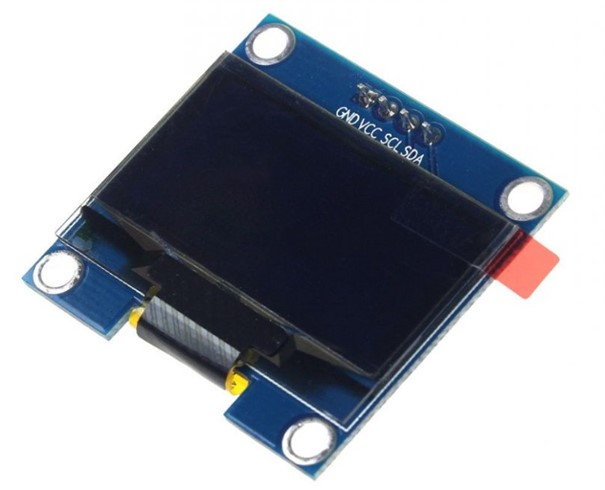
\includegraphics[width=5.4cm]{images/komponenty/displej.jpg}
	\caption{OLED displej \cite{dratek_web}}
\end{figure}

\section{Hlasový modul}
O~průběhu měření je měřič informován kromě displeje i pomocí reproduktoru, tak aby nemusel při měření sledovat displej. Měřiče o~průběhu měření informují slovní pokyny „Čas byl synchronizován“ a „Měření času bylo uloženo“, které byly vytvořeny pomocí převodu textu na mp3 soubor. Jelikož Arduino neumožňuje ukládat žádné soubory do své vnitřní paměti, tak jsou mp3 soubory se zvukovými informacemi nahrány na Micro SD kartu. Soubory jsou z~Micro SD karty čteny pomocí hlasového modulu a přehrávány pomocí reproduktoru, který je k~hlasovému modulu připojen. Hlasový modul s~Arduinem komunikuje prostřednictvím sériové komunikace \cite{arduino_navody}.

\begin{figure}[H]
	\centering
	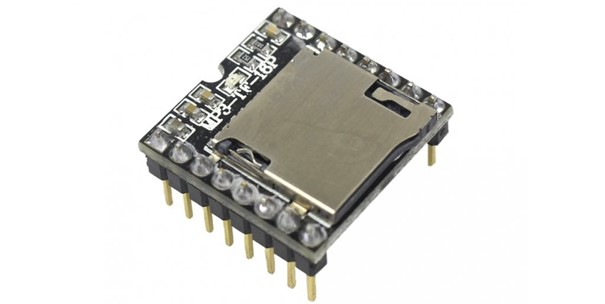
\includegraphics[width=7cm]{images/komponenty/DF_Player.jpg}
	\caption{Hlasový modul \cite{laskakit_web}}
\end{figure}

\begin{figure}[H]
	\centering
	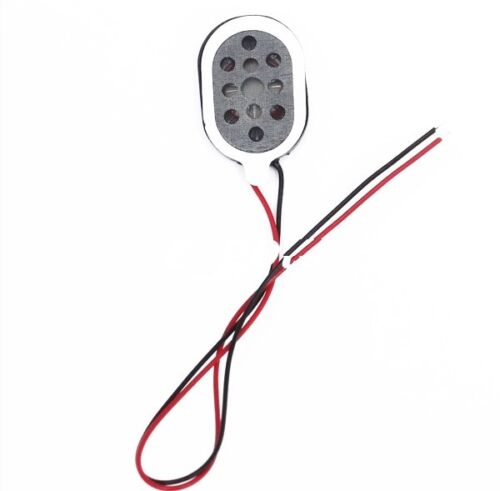
\includegraphics[width=4cm]{images/komponenty/reproduktor.jpg}
	\caption{Reproduktor \cite{arduino}}
\end{figure}

\section{RGB LED}
Kromě displeje a zvukového signálu je měřič informován o~průběhu měření také prostřednictvím elektroluminiscenční diody (\zk{LED}, z~anglického Light Emitting Diode). Jako \zkratka{LED} je využit modul RGB \zk{LED}, který se skládá ze tří samostatných \zk{LED} (červená, zelená, modrá). Tyto \zk{LED} mají společnou \text{katodu}, ale samostatné anody. K ovládání jasu jednotlivých barev slouží \zkratka{PWM}. Jednotlivé anody lze nezávisle na sobě připojit na piny s podporou \zk{PWM}, což umožňuje ovládat samostatně jednotlivé barvy. Další výhodou tohoto modulu je, že již má integrované ochranné rezistory. Během měření může \zk{LED} signalizovat různé stavy: Nejprve bliká červeně v~každý okamžik, kdy přijme signál DCF77 (v~ideálním případě je to jednou za sekundu). Ve chvíli, kdy je čas poprvé synchronizován se změní červené blikání na zelené, což informuje měřiče o~úspěšné synchronizaci času. Dále \zk{LED} bliká modře v~každý okamžik, kdy měřič provede měření \cite{arduino_navody}.
\begin{figure}[H]
	\centering
	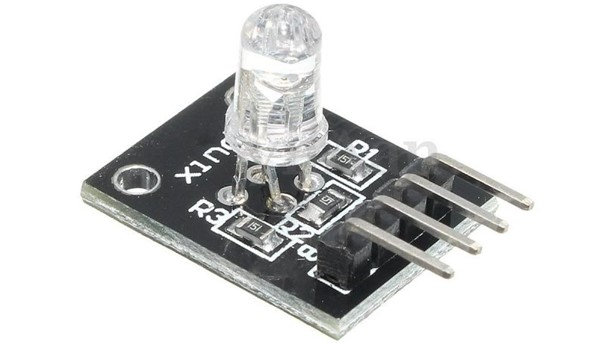
\includegraphics[width=6cm]{images/komponenty/RGB_LED.jpg}
	\caption{Modul s~RGB LED \cite{dratek_web}}
\end{figure}

\section{Převodník TTL na RS232}
Aby byl spolu s~časovými údaji uložen na Micro SD kartu vodorovný směr (a případně i zenitový úhel) měřený totální stanicí, je potřeba zajistit komunikaci Arduina s~totální stanicí. K~tomu lze využít sériovou komunikaci pomocí UART. Konkrétně byla využita totální stanice Leica TC1700. Ta využívá pro sériovou komunikaci standart RS-232 a lze k~ní tedy připojit sériový kabel RS-232 \cite{tps-dna}. Standart RS-232 využívá pro datové signály +3~V až +25~V jako logickou nulu a -3~V až -25~V jako logickou jedničku. Arduino UNO využívá protokol TTL, který považuje hodnoty okolo 0~V za logickou nulu a hodnoty v~okolí +5~V za logickou jedničku. Aby mohl být kabel RS-232 připojen i k~Arduinu, je potřeba využít převodník TTL na RS-232 \cite{sparkfun-tutorial}.

\begin{figure}[H]
	\centering
	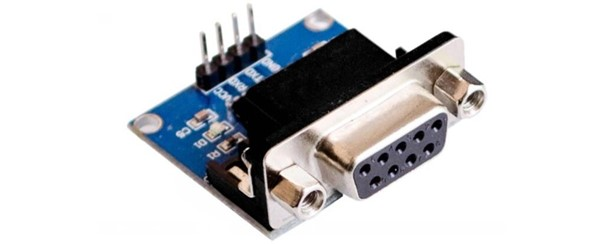
\includegraphics[width=8.5cm]{images/komponenty/prevodnik.jpg}
	\caption{Převodník TTL na RS232 \cite{laskakit_web}}
\end{figure}

\section{Bluetooth modul}
Pro export dat z~Micro SD karty, aniž by bylo potřeba ji vyjmout, lze využít \text{Bluetooth} modul. Konkrétně byl pro tento účel využit modul HC-05. Tento modul využívá sériovou komunikaci pomocí UART a podporuje Bluetooth ve verzi 2.0. Pomocí Bluetooth modulu lze přenášet binární data. Modul je připojen pomocí pinů GND, VCC, RX a TX. Kromě toho obsahuje piny STATE a EN, které slouží pro konfiguraci modulu. Pin EN na modulu HC-05 umožňuje přepnutí modulu do režimu „enabled“. V~tomto režimu lze pomocí AT příkazů nastavit jméno, heslo, popřípadě i baud rate a další parametry modulu \cite{arduino_navody}.

\begin{figure}[H]
	\centering
	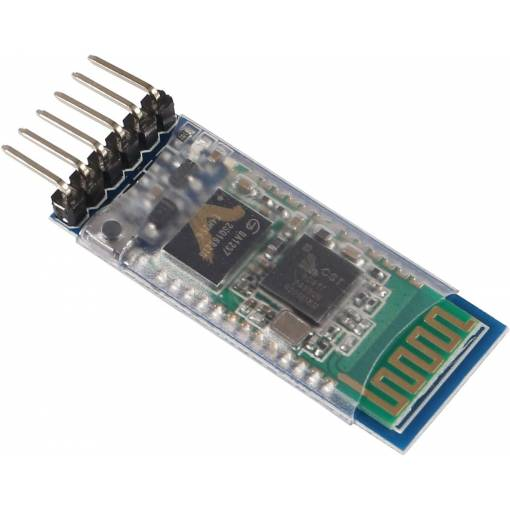
\includegraphics[width=4.6cm]{images/komponenty/BLUETOOTH-HC05.jpg}
	\caption{Bluetooth modul HC-05 \cite{dratek_web}}
\end{figure}

\section{Deska plošných spojů}
Během vývoje zařízení byly všechny komponenty spojovány pomocí kabelů. Nevýho\-dou propojení pomocí kabelů je velká prostorová náročnost a celková nepřehlednost. Z~toho důvodu bývá obvykle propojení různých komponentů realizováno pomocí desky plošných spojů. Pro snadné propojení všech využitých komponentů byla tedy vyhotovena \zkratka{DPS}.

\begin{figure}[H]
	\centering
	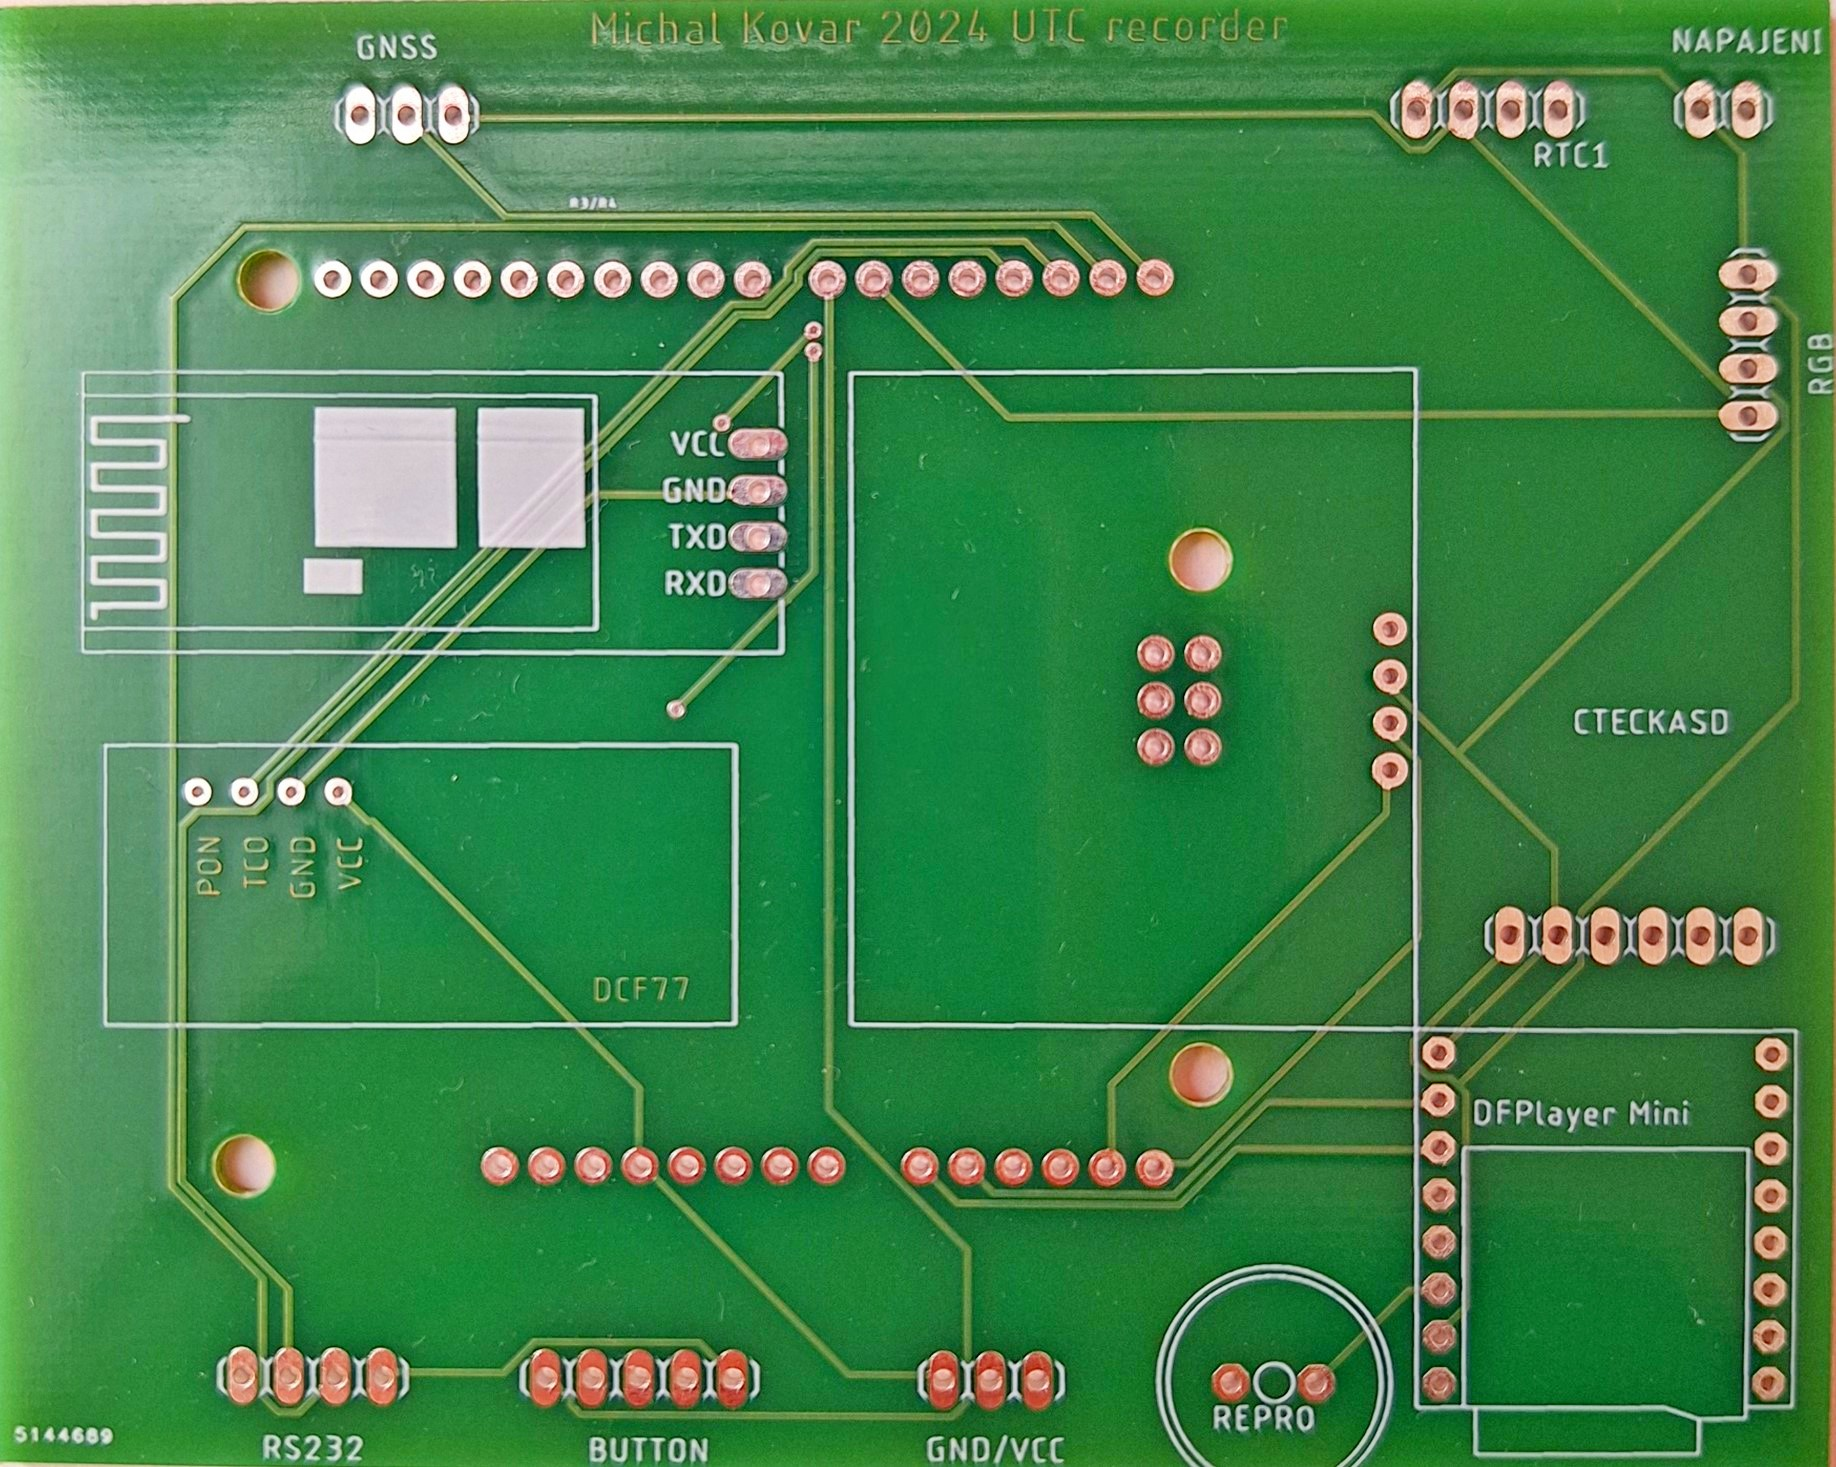
\includegraphics[width=5cm]{images/komponenty/dps_foto.jpg}
	\caption{Výsledná DPS}
\end{figure}

\section{Cena komponentů}
Ceny jednotlivých komponentů se mění v čase a mohou se lišit v závislosti na místě (obchodě), kde byly zakoupeny. Cena výsledného zařízení závisí na tom, zda byly použity všechny komponenty pro plnou funkcionalitu, nebo zda byly některé funkce vynechány.  Pokud se zařízení vyrábí s omezenou funkcionalitou, lze využít levnější Arduino UNO R3. Náklady na výsledné zařízení lze také snížit použitím „klonů“ místo originálního Arduina. Níže uvedená tabulka obsahuje komponenty potřebné pro zařízení s plnou funkcionalitou a uvádí ceny, za které byly tyto komponenty zakoupeny.

\begin{table}[H]
    \centering
    \caption{Cena použitých součástek}
    \begin{tabular}{|c|c|c|}
    \hline
    \textbf{Název} & \textbf{Cena} & \textbf{Odkaz na obchod}\\
    \hline\hline
    Arduino UNO R4 WiFi         & 768 Kč            & \href{https://www.laskakit.cz/arduino-uno-r4-wifi--original/}{laskakit.cz}  \\ \hline
    Přijímač DCF77              & 5,60 \euro/140 Kč  & \href{https://www.pollin.de/p/dcf-empfangsmodul-dcf1-810054}{pollin.de} \\ \hline
    Přijímač GNSS               & 339 Kč            & \href{https://dratek.cz/arduino/1733-gps-satelitni-urceni-polohy-neo-7m-modul.html?}{dratek.cz} \\ \hline
    Čtečka Micro SD karet       & 24 Kč             & \href{https://dratek.cz/arduino/993-ctecka-microsd-karet.html?}{dratek.cz} \\ \hline
    Tlačítko (rotační enkodér)   & 38 Kč             & \href{https://dratek.cz/arduino/837-rotacni-enkoder.html?}{dratek.cz} \\ \hline
    OLED displej                & 167 Kč            & \href{https://dratek.cz/arduino/3181-iic-i2c-oled-1-3-displej-128x64-bily.html?}{dratek.cz} \\ \hline
    Hlasový modul               & 66 Kč             & \href{https://dratek.cz/arduino/4857-hlasovy-modul-s-integrovanym-mp3-prehravacem-dfplayer.html?}{dratek.cz} \\ \hline
    Reproduktor                 & 19 Kč             & \href{https://dratek.cz/arduino/1175-reproduktor-1w-8ohm.html?}{dratek.cz} \\ \hline
    RGB LED                     & 15 Kč             & \href{https://dratek.cz/arduino/837-rotacni-enkoder.html}{dratek.cz} \\ \hline
    Bluetooth modul HC-05       & 117 Kč            & \href{https://dratek.cz/arduino/1005-bluetooth-modul-hc-05.html?}{dratek.cz} \\ \hline
    Deska plošných spojů        & 9,34 \$/216 Kč    & \href{https://www.allpcb.com/}{allpcb.com} \\ \hline
     \textbf{Celkem}            & 1909 Kč           & - \\ \hline
    \end{tabular}\\
\end{table}


